%!TEX root = MemoireZelliges.tex

\begin{center}
\thispagestyle{empty}

{\LARGE
Programme PACT ARCHI-MED Glaçures -- II\par
}

% \vspace*{-0.75\baselineskip}

\rule{.5\textwidth}{1pt}

% \bigskip

{\bfseries\huge
\MakeUppercase{Contribution à la réhabilitation architecturale du 
\PaM, Meknès, Maroc, \siecle{xvii}}

\bigskip

Recherche des caractéristiques physiques de zelliges de pavement
}

\vfill

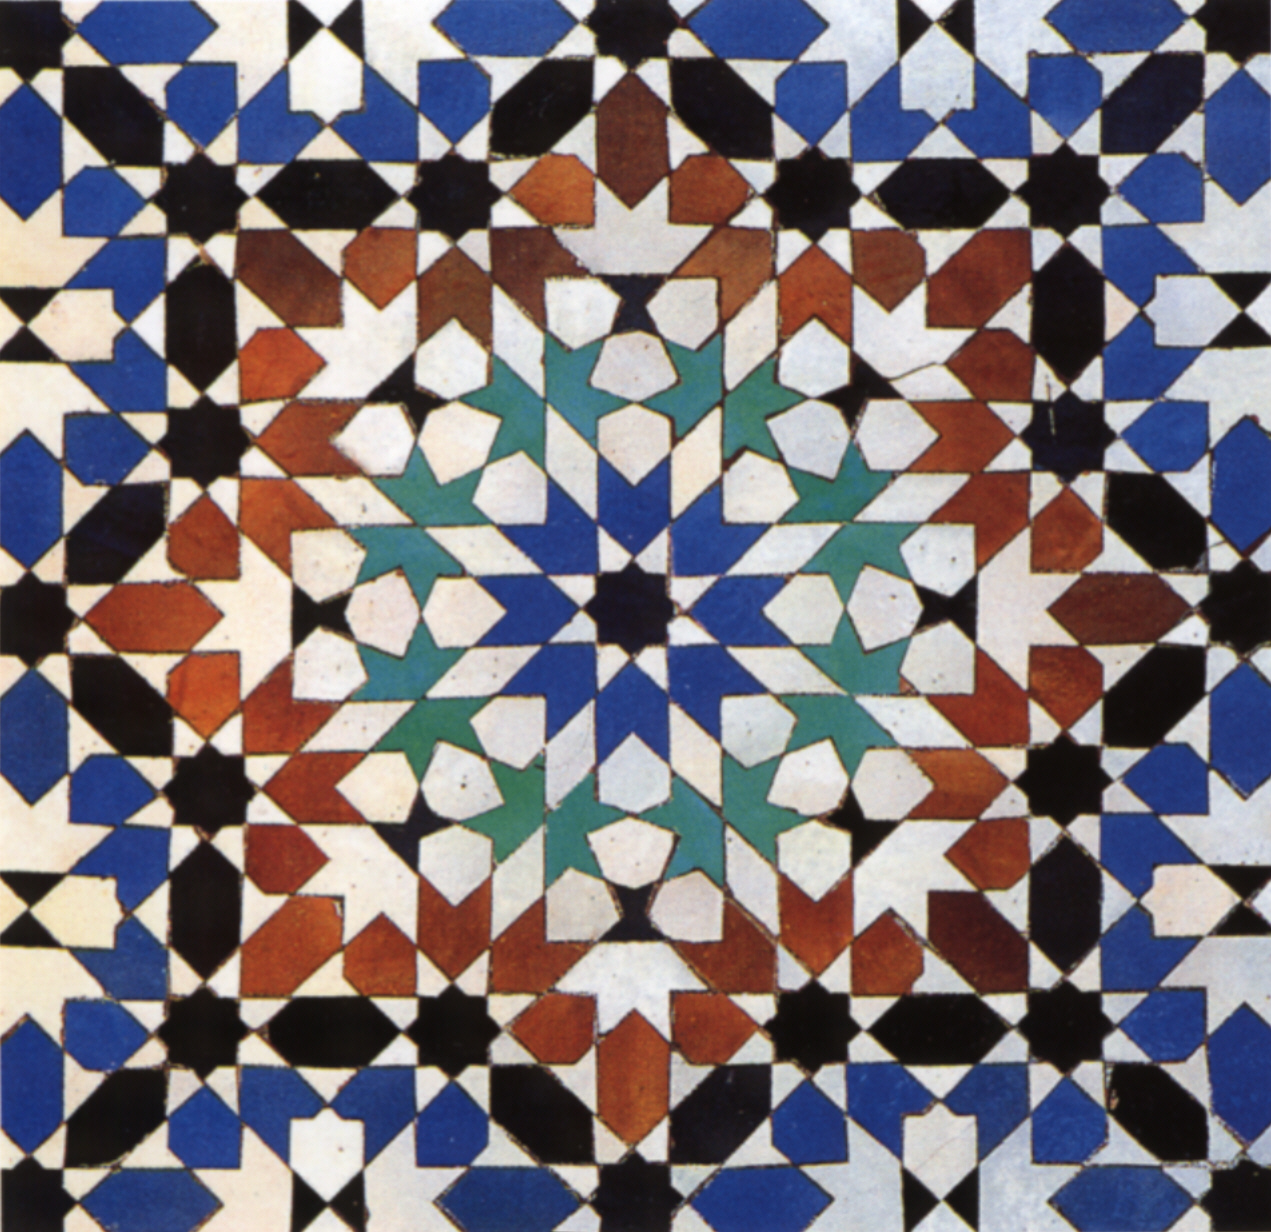
\includegraphics[width=10cm]{zellige_01}

\vfill

\textbf{\Large LABETOULE Sonia}

{\itshape
Maître ès Sciences \par
(Chimie physique) \par
}

\vfill

\framebox[\textwidth]{\small Juin~2000 \hfill MÉMOIRES DE LA SÉRIE 
\textbf{\frquote{FORMATION À ET PAR LA RECHERCHE}} \hfill \no441. DESS}
\end{center}



% {\centering Programme PACT ARCHI-MED Glaçures -- II \par}

% {\centering [Warning: Draw object ignored]\par}

% {\centering \textbf{CONTRIBUTION A LA REHABILITATION ARCHITECTURALE DU PALAIS~AL-MANSOUR, MEKNES, MAROC, XVII\ieme s.} \par}


% {\centering\bfseries Recherche des caractéristiques physiques de zelliges de pavement \par}

% {\centering\bfseries LABETOULE Sonia \par}

% {\centering\itshape Maître ès Sciences \par}

% {\centering\itshape (Chimie physique) \par}









\clearpage

\begin{RaggedLeft}
  \itshape
  \frquote{\dots du savoir ce n'est qu'une petite part que nous 
  t'avons octroyé, ô homme}

  (Saint Qur'an
\end{RaggedLeft}


{\raggedleft\itshape À Frédéric \par}


\chapter*{Remerciements}
\addcontentsline{toc}{chapter}{Remerciements}
%======================================================================

Je tiens à remercier Madame le Professeur Françoise~\bsc{Bechtel}, 
directrice du \emph{Centre de Recherche en Physique Appliquée à 
l'Archéologie}, et Monsieur le Professeur Max~\bsc{Schv{\oe}rer} 
de m'avoir accueillie dans leur laboratoire.

\bigskip

Merci également à Ayed~\bsc{Ben Amara}, qui m'a encadrée lors de ce 
stage, pour son infinie patience et sa grande disponibilité durant 
ces quelques mois.

\bigskip

Un grand merci à l'ensemble des membres du laboratoire, permanents, 
doctorants et étudiants, pour leur aide précieuse et leur gentillesse 
tout au long de cette année.

\bigskip

Et un merci tout particulier à Frédéric qui m'a soutenue, aidée, 
encouragée et surtout subie pendant toutes les étapes de mon stage 
et de la réalisation de ce mémoire.

\chapter*{Avant-propos}
\addcontentsline{toc}{chapter}{Avant-propos}
%======================================================================

Les procédés nécessaires à la réalisation de glaçures sur céramique 
remonte à la plus haute Antiquité, probablement au moins 
\num{5000}~ans avant~J.C. Ce matériau a été et est toujours utilisé 
pour produire de la vaisselle, des objets de parure ou d'hygiène, 
des jeux et instruments de musique, et pour protéger et décorer 
l'architecture. On peut dire que la céramique en général et la 
céramique glaçurée en particulier est l'une des formes d'expression 
artistique les plus importantes de l'humanité et l'une de ses plus 
grandes réussites technologiques. C'est sur elle que se sont basés les 
archéologues pour établir leurs chronologies, c'est grâce à certains 
de ses décors (sur les vases grecs par exemple) que l'on peut 
reconstituer les modes de vie anciens. L'étude de la céramique 
glaçurée est donc un des aspects fondamentaux de l'archéologie.

Mon stage de troisième cycle s'est déroulé au \emph{Centre de 
Recherche en Physique Appliquée à l'Archéologie} (CRPAA) de 
l'université Bordeaux~I, laboratoire qui s'est depuis longtemps 
spécialisé dans l'étude de ce matériau.

J'ai effectué ce travail dans le cadre du programme de coopération 
internationale PACT ARCHI-MED (archéomatériaux composites de 
l'architecture en Méditerranée : verre-terre cuite -- altération et 
recréation) associant la Turquie (Université d'Istanbul), l'Espagne 
(Musée de céramique de Manises), Le Maroc (Université Moulay Ismail 
de Meknès) et la France (CRPAA). Ce programme a pour but l'étude des 
céramiques glaçurées architecturales du monde méditerranéen avec deux 
objectifs distincts :

\begin{itemize}
  \item \emph{Altérations} : mettre au point des techniques 
        permettant d'établir un diagnostic des altérations, 
        d'en identifier les causes probables, de déterminer les 
        caractéristiques (textures, compositions) favorisant 
        l'altération ou une meilleure résistance aux agents extérieurs.
  \item \emph{Reproduction} : retrouver les techniques anciennes 
        permettent de recréer certains types de décors, de contrôler 
        couleur, texture et composition des matériaux de recréation, 
        d'optimiser les caractéristiques des matériaux de substitution 
        qui déterminent leur résistance aux agents extérieurs.
\end{itemize}

L'objet de mon stage était plus précisément l'étude physico-chimique 
d'échantillons marocains -- des zelliges -- provenant du \PaM de 
Meknès, datés du \siecle{xvii}.

Trois autres études sur des zelliges se sont déroulées en parallèle au 
laboratoire :

\begin{itemize}
  \item échantillons du Palais de Chellah (Rabat), 
        \siecle{xiv} (Jennifer~\bsc{Delmas}, maîtrise) ;
  \item échantillons de la medersa Filalia (Meknès), 
        \siecle{xiv} (Richard~\bsc{Cheret}, DESS) ;
  \item échantillons de la medersa Bu'Inaniya (Meknès), 
        \siecle{xiv} (Yannick~\bsc{Melin}, maîtrise et 
        Richard~\bsc{Cheret}, DESS).
\end{itemize}

Outre la caractérisation de ce matériel céramique, l'intérêt de ce 
stage de DESS réside aussi dans l'apprentissage et l'acquisition 
d'une autonomie d'utilisation des différentes techniques d'analyse 
physico-chimiques mises en {\oe}uvre au laboratoire : \MEB[ie], 
\EDS, \CL, \SAO, \DX.